\chapter{Bayesian Estimation}\label{sec:Bayesian_estimation}

\vfill
\localtableofcontents
\vfill
\newpage

\section{Introduction}

The goal of this chapter is to formally introduce the tools necessary to solve the general filtering problem. More precisely, given a dynamical system whose state evolves according to a known stochastic model and is partially observed through noisy measurements, we seek to sequentially estimate the system state at each time step in an optimal sense. We first define what optimality means in a rigorous setting, then derive exact and approximate solutions to this problem. We also discuss the limitations of such methods.

Formally, for $d_x,d_z,d_{\varphi}\in\mathbb{N}^*$, we consider a hidden Markov chain $(x_k)_{k\geq0}$ taking values in $\mathbb{R}^{d_x}$ and a series of observations $(z_k)_{k\geq1}$ taking values in $\mathbb{R}^{d_z}$, each associated with the unknown state $x_k$. The quantity of interest is a mapping of the state under a known function $\varphi:\mathbb{R}^{d_x}\to\mathbb{R}^{d_{\varphi}}$, which allows us to target any derived quantity of the state (\textit{e.g.} position, velocity, or a subset of coordinates). When solving a navigation problem, the state and observation processes are linked by the state-space model \cite{bib:HMM}:
\begin{equation}
	\left\{\begin{aligned}
	x_k&=f_k(x_{k-1},w_k)\\
	z_k&=h_k(x_k,n_k)
	\end{aligned}\right.\label{eq:navigation_problem}
\end{equation}
where the processes $w_k\in\mathbb{R}^{d_w}$ and $n_k\in\mathbb{R}^{d_n}$ denote the evolution and observation noises respectively, and are assumed to be white noises (\textit{i.e.} temporally independent, centered noises of finite variance), mutually independent and independent of $x_0$.

The known data of this problem are:
\begin{equation}
	\left\{\begin{array}{ll}
	p_0&\text{the probability density of the initial state }x_0\\
	f_k&\text{the evolution function}\\
	p_k^{(e)}&\text{the probability density of the evolution noise }w_k\\
	z_k&\text{the current noisy observation}\\
	h_k&\text{the observation function}\\
	p_k^{(o)}&\text{the probability density of the observation noise }n_k
	\end{array}\right.
\end{equation}

\begin{remark}[Control input]
	In many navigation applications, a control input $u_k$ is also available, and the evolution function takes the form $f_k(x_{k-1}, u_k, w_k)$. For the sake of clarity, we omit $u_k$ from the general formulation as it can always be absorbed into $f_k$ or treated as a known deterministic input.
\end{remark}

Depending on how observations are used relative to the time index of the state to estimate, three problems arise \cite{bib:nonlinear-smoothing}:
\begin{itemize}
	\item \textbf{Filtering:} estimate $\varphi(x_k)$ given $\mathbf{z}_{1:k}\triangleq(z_1,\dots,z_k)$. It is the most common case in real-time navigation.
	\item \textbf{Smoothing:} estimate $\varphi(x_l)$ for $l < k$ given $\mathbf{z}_{1:k}$. It corresponds to refining past estimates using future observations.
	\item \textbf{Prediction:} estimate $\varphi(x_l)$ for $l > k$ given $\mathbf{z}_{1:k}$. This amounts to anticipating future states from current observations.
\end{itemize}

This thesis focuses on the filtering problem. The rest of this chapter is organised as follows:
\begin{itemize}
	\item\Cref{sec:state_estimation} rigorously defines what it means to optimally estimate $\varphi(x_k)$ from the observations $\mathbf{z}_{1:k}$, and shows that all classical optimality criteria reduce to computing the posterior probability density function (PDF) $p(x_k|\mathbf{z}_{1:k})$.
	\item\Cref{sec:analytical_estimation} derives analytical filtering algorithms to propagate this density over time, and discusses their limitations.
	\item\Cref{sec:Monte_Carlo} then presents asymptotically optimal numerical methods based on Monte Carlo (MC) sampling that alleviate such flaws.
	\item Finally, \cref{sec:particle_filtering} presents advanced particle filtering methods that improve upon standard MC techniques.
\end{itemize}

\section{State Estimation}\label{sec:state_estimation}

The first issue to tackle is to define precisely the meaning of "best estimator" of $\varphi(x_k)$ given $\mathbf{z}_{1:k}$ \cite{bib:Bayesian-estimators}. Formally, given a functional metric space $(\mathcal{F},\rho)$, it amounts to finding a measurable function $\psi\in\mathcal{F}$ that minimises the expected loss:
\begin{equation}
	\underset{\psi\in\mathcal{F}}{\operatorname{argmin}}(\rho(\psi(\mathbf{z}_{1:k}),\varphi(x_k)))\label{eq:loss_function_with_k}
\end{equation}

Depending on the considered space and distance, different optimal estimators arise. We present three classical ones below. For the sake of simplicity, we write $Z$ for a generic observation vector and $X$ for the underlying state, as opposed to the time-indexed processes $x_k$ and $z_k$. At a fixed time step $k$, \eqref{eq:loss_function_with_k} thus becomes:
\begin{equation}
	\underset{\psi\in\mathcal{F}}{\operatorname{argmin}}(\rho(\psi(Z),\varphi(X)))\label{eq:loss_function}
\end{equation}

For the remainder of this document, we let, for $d,d',p\in\mathbb{N}^*$:
\begin{equation}
	\begin{aligned}
	\mathcal{L}^0\left(\mathbb{R}^{d'},\mathbb{R}^{d}\right)&\triangleq\left\{f:\mathbb{R}^{d'}\to\mathbb{R}^{d}\:\middle|\:f\text{ measurable}\right\}\\
	\mathcal{L}^p\left(\mathbb{R}^{d}\right)&\triangleq\left\{A\text{ an }\mathbb{R}^{d}\text{-valued random variable}\:\middle|\:\mathbb{E}\left[\|A\|^p\right]<\infty\right\}
	\end{aligned}
\end{equation}
where almost surely equal random variables are identified.

\subsection{Posterior Expectation Estimator}

Let:
\begin{equation}
	\mathcal{F}\triangleq\left\{\psi\in\mathcal{L}^0\left(\mathbb{R}^{d_z},\mathbb{R}^{d_{\varphi}}\right)\:\middle|\:\mathbb{E}\left[\|\psi(Z)\|^2\right]<\infty\right\}
\end{equation}
To simplify notations, we identify each estimator $\psi\in\mathcal{F}$ with the random variable $\psi(Z)$ it produces. Under this identification, $\mathcal{F}$ is a closed subspace of $\mathcal{L}^2\left(\mathbb{R}^{d_{\varphi}}\right)$, and can be equipped with the inner product:
\begin{equation}
	(A,B)\in\mathcal{F}^2\mapsto\langle A|B\rangle\triangleq\mathbb{E}\left[A(Z)^\top B(Z)\right]
\end{equation}
where $\mathbb{E}[X]$ denotes the expectation of the random variable $X$.

Let $\|\cdot\|$ be the norm associated with $\langle\cdot|\cdot\rangle$. When $\varphi(X)\in\mathcal{L}^2\left(\mathbb{R}^{d_{\varphi}}\right)$, the minimisation problem \eqref{eq:loss_function} is equivalent to:
\begin{equation}
	\underset{\psi\in\mathcal{F}}{\operatorname{argmin}}\left(\mathbb{E}\left[\|\psi(Z)-\varphi(X)\|^2\right]\right)\label{eq:MMSE_problem}
\end{equation}

An estimator solving \eqref{eq:MMSE_problem} is called a minimum mean squared error (MMSE) estimator.

\begin{proposition}[MMSE estimator]\label{th:MMSE_estimator}
	The unique solution to \eqref{eq:MMSE_problem} is the posterior expectation:
	\begin{equation}
		\hat{\psi}_{\mathrm{MMSE}}(z)\triangleq\mathbb{E}[\varphi(X)|Z=z]
	\end{equation}
\end{proposition}

\begin{proof}
	Let $\hat{\psi}(z)\triangleq\mathbb{E}[\varphi(X)|Z=z]$ and $\psi\in\mathcal{F}$. It comes that:
	\begin{equation}
		\begin{aligned}
		\rho(\psi(Z),\varphi(X))^2&=\langle\psi(Z)-\varphi(X)|\psi(Z)-\varphi(X)\rangle\\
		&=\langle\psi(Z)-\hat{\psi}(Z)+\hat{\psi}(Z)-\varphi(X)|\psi(Z)-\hat{\psi}(Z)+\hat{\psi}(Z)-\varphi(X)\rangle\\
		&=\langle\psi(Z)-\hat{\psi}(Z)|\psi(Z)-\hat{\psi}(Z)\rangle+\langle\hat{\psi}(Z)-\varphi(X)|\hat{\psi}(Z)-\varphi(X)\rangle\\
		&\qquad+2\langle\psi(Z)-\hat{\psi}(Z)|\hat{\psi}(Z)-\varphi(X)\rangle
		\end{aligned}
	\end{equation}

	The cross term vanishes by the tower property of conditional expectation:
	\begin{equation}
		\begin{aligned}
		\langle\psi(Z)-\hat{\psi}(Z)|\hat{\psi}(Z)-\varphi(X)\rangle&=\mathbb{E}\left[(\psi(Z)-\hat{\psi}(Z))^\top(\hat{\psi}(Z)-\varphi(X))\right]\\
		&=\iint{(\psi(z)-\hat{\psi}(z))^\top(\hat{\psi}(z)-\varphi(x))\:p(dx,dz)}\\
		&=\iint{(\psi(z)-\hat{\psi}(z))^\top(\hat{\psi}(z)-\varphi(x))\:p(dx|z)\:p(dz)}\\
		&=\int{(\psi(z)-\hat\psi(z))^\top\left(\int{(\hat\psi(z)-\varphi(x))\:p(dx|z)}\right)\:p(dz)}\hspace{-4pt}\\
		&=\int{(\psi(z)-\hat\psi(z))^\top\left(\hat\psi(z)-\mathbb{E}[\varphi(X)|Z=z]\right)\:p(dz)}\\
		&=\int{(\psi(z)-\hat\psi(z))^\top\times0\:p(dz)}\\
		&=0
		\end{aligned}
	\end{equation}
	by definition of $\hat\psi(z)$.

	Therefore:
	\begin{equation}
		\begin{aligned}
		\rho(\psi(Z),\varphi(X))^2&=\rho(\psi(Z),\hat{\psi}(Z))^2+\rho(\hat{\psi}(Z),\varphi(X))^2\\
		&\geq\rho(\hat{\psi}(Z),\varphi(X))^2
		\end{aligned}
	\end{equation}
	with equality if and only if $\|\psi(Z)-\hat{\psi}(Z)\|^2=0$, \textit{i.e.} $\psi=\hat{\psi}$ almost surely (a.s.).
\end{proof}

\begin{remark}[Geometric interpretation]
	The MMSE estimator is the orthogonal projection of $\varphi(X)$ onto $\mathcal{F}$, viewed as a closed subspace of $\mathcal{L}^2\left(\mathbb{R}^{d_{\varphi}}\right)$, \textit{i.e.} the set of all square-integrable random variables that are measurable with respect to $Z$. The disappearance of the cross term in the proof above is precisely the orthogonality condition characterising this projection.
\end{remark}

\begin{remark}[MMSE assumptions]
	Square-integrability of $\varphi(X)$ is only required for the minimisation \eqref{eq:MMSE_problem} to be well-posed, not the estimator itself. The posterior expectation $\mathbb{E}[\varphi(X)|Z=z]$ remains well-defined for any $\varphi(X)\in\mathcal{L}^1\left(\mathbb{R}^{d_{\varphi}}\right)$, but it only minimises the mean squared error inside of $\mathcal{L}^2\left(\mathbb{R}^{d_{\varphi}}\right)$.
\end{remark}

\subsection{Posterior Median Estimator}

Because the MMSE estimator minimises a quadratic loss, it is highly sensitive to extreme values and may perform poorly for heavy-tailed distributions. To mitigate this sensitivity to outliers, one can use an absolute loss instead. In dimension $d_{\varphi}=1$, let:
\begin{equation}
	\mathcal{F}\triangleq\left\{\psi\in\mathcal{L}^0\left(\mathbb{R}^{d_z},\mathbb{R}\right)\:\middle|\:\mathbb{E}[|\psi(Z)|]<\infty\right\}
\end{equation}

As previously, $\mathcal{F}$ is identified as a subspace of $\mathcal{L}^1(\mathbb{R})$, and is equipped with the following non-Euclidean distance:
\begin{equation}
	(A,B)\in\mathcal{F}^2\mapsto\rho(A,B)\triangleq\mathbb{E}[|A(Z)-B(Z)|]
\end{equation}

The minimisation problem \eqref{eq:loss_function} thus becomes:
\begin{equation}
	\underset{\psi\in\mathcal{F}}{\operatorname{argmin}}(\mathbb{E}[|\psi(Z)-\varphi(X)|])\label{eq:median_problem}
\end{equation}

While the terminology is less standard than MMSE, an estimator solving \eqref{eq:median_problem} is often called a minimum mean absolute error (MMAE) estimator.

\begin{proposition}[MMAE estimator, simplified assumptions]
	Assume that, for every $z$, the conditional distribution of $\varphi(X)$ given $Z=z$ is absolutely continuous with a strictly positive density. Then, the unique solution to \eqref{eq:median_problem} is the posterior median of $\varphi(X)$ given $Z=z$, \textit{i.e.} the value $\hat{\psi}_{\mathrm{MMAE}}(z)\in\mathbb{R}$ that satisfies:
	\begin{equation}
		\mathbb{P}\left(\varphi(X)\geq\hat{\psi}_{\mathrm{MMAE}}(z)|Z=z\right)=\mathbb{P}\left(\varphi(X)<\hat{\psi}_{\mathrm{MMAE}}(z)|Z=z\right)=\frac{1}{2}\label{eq:median_estimator}
	\end{equation}
\end{proposition}

\begin{proof}
	By the law of total expectation, for any $\psi\in\mathcal{F}$, we have:
	\begin{equation}
		\mathbb{E}[|\psi(Z)-\varphi(X)|]=\mathbb{E}\left[\int{|\psi(z)-\varphi(x)|\:p(dx|Z=z)}\right]
	\end{equation}

	Since the outer expectation is over non-negative quantities, this is minimised by minimising the inner integral pointwise for each $z$, \textit{i.e.} by solving:
	\begin{equation}
		\underset{u\in\mathbb{R}}{\operatorname{argmin}}\int{|\varphi(x)-u|\:p(dx|Z=z)}
	\end{equation}

	As $u\mapsto|\varphi(x)-u|$ is convex, so is the integral, hence any stationary point is a global minimum. Since the conditional law is absolutely continuous, the integral is differentiable in $u$. By differentiating this expression with respect to $u\in\mathbb{R}$, it follows that:
	\begin{equation}
		\begin{aligned}
		&\frac{d}{du}\left(\int{|\varphi(x)-u|\:p(dx|Z=z)}\right)=0\\
		\iff\quad&\frac{d}{du}\left(\int{\left((\varphi(x)-u)\:\mathbbm{1}_{\varphi(x)\geq u}(x)-(\varphi(x)-u)\:\mathbbm{1}_{\varphi(x)<u}(x)\right)\:p(dx|Z=z)}\right)=0\\
		\iff\quad&\int{\left(-\mathbbm{1}_{\varphi(x)\geq u}(x)+\mathbbm{1}_{\varphi(x)<u}(x)\right)\:p(dx|Z=z)}=0\\
		\iff\quad&\mathbb{P}(\varphi(X)\geq u|Z=z)=\mathbb{P}(\varphi(X)<u|Z=z)
		\end{aligned}
	\end{equation}

	Since the total probability is one, this is equivalent to $u=\hat{\psi}_{\mathrm{MMAE}}(z)$ as defined in \eqref{eq:median_estimator}, with the strict positivity of the density ensuring uniqueness.
\end{proof}

\begin{remark}[Median assumptions]
	The absolute continuity and positivity assumptions are only required for the clean statement above, not for the existence of a solution. Since the inner integral is convex, continuous and coercive in $u$, a minimum always exists for any integrable conditional distribution. In full generality, the set of solutions is the closed interval of medians:
	\begin{equation}
		\left\{u\in\mathbb{R}\:\middle|\:\mathbb{P}(\varphi(X)\leq u|Z=z)\geq\frac{1}{2}\text{ and }\mathbb{P}(\varphi(X)\geq u|Z=z)\geq\frac{1}{2}\right\}
	\end{equation}
	The absence of atoms then guarantees that this interval is characterised by the equality \eqref{eq:median_estimator}, while the strict positivity of the density ensures that it reduces to a single point.
\end{remark}

\begin{remark}[Generalised median]
	The extension to higher dimensions $d_{\varphi}>1$ is non-trivial. The $\mathcal{L}^1\left(\mathbb{R}^{d_{\varphi}}\right)$ median, also called geometric median, is the most common generalisation. In the remainder of this thesis, we focus on the MMSE and MAP estimators (presented below), which extend naturally to any dimension.
\end{remark}

\subsection{Maximum \textit{a Posteriori} Estimator}

As they produce a single point estimate that may lie in a low-probability region, both the MMSE and the MMAE estimators may not be suited for multimodal posteriors. In such cases, a natural alternative is to select a maximum of the posterior density.

Let $\mathcal{F}\triangleq\mathcal{L}^0\left(\mathbb{R}^{d_z},\mathbb{R}^{d_{\varphi}}\right)$, with no integrability constraint. The maximum \textit{a posteriori} (MAP) estimator is defined as the global mode of the posterior density of $\varphi(X)$:
\begin{equation}
	\hat{\psi}_{\mathrm{MAP}}\triangleq\underset{\psi\in\mathcal{F}}{\operatorname{argmax}}\left(\mathbb{E}\left[p_{\varphi(X)|Z}(\psi(Z)|Z)\right]\right)
\end{equation}

As the objective is separable over $z$, the maximisation can be carried out pointwise, yielding for each $z$:
\begin{equation}
	\hat{\psi}_{\mathrm{MAP}}(z)=\underset{u\in\mathbb{R}^{d_{\varphi}}}{\operatorname{argmax}}\left(p_{\varphi(X)|Z}(u|z)\right)
\end{equation}

Using Bayes' theorem, this is equivalent to:
\begin{equation}
	\hat{\psi}_{\mathrm{MAP}}(z)=\underset{u\in\mathbb{R}^{d_{\varphi}}}{\operatorname{argmax}}\left(p_{Z|\varphi(X)}(z|u)\:p_{\varphi(X)}(u)\right)\label{eq:MAP_Bayes}
\end{equation}
since the normalising constant $p_Z(z)$ is independent of $u$.

Although the MAP estimator avoids low-density regions, it still reduces the posterior to a single point. In particular, in multimodal situations, only one mode is retained, while the remaining ones are discarded.

\begin{remark}[MAP optimisation problem]
	The MAP estimator can be seen as the solution of an optimisation problem of the form \eqref{eq:loss_function}, associated with the threshold loss:
	\begin{equation}
		\forall\varepsilon>0,\:(A,B)\in\mathcal{F}^2\mapsto\rho_\varepsilon(A,B)\triangleq\mathbbm{1}_{\|A(Z)-B(Z)\|>\varepsilon}
	\end{equation}
	in the limit $\varepsilon\to0^+$:
	\begin{equation}
		\hat{\psi}_{\mathrm{MAP}}=\lim_{\varepsilon\to0^+}\ \underset{\psi\in\mathcal{F}}{\operatorname{argmin}}(\rho_\varepsilon(\psi(Z),\varphi(X)))
	\end{equation}
\end{remark}

\subsubsection{Maximum Likelihood Estimator}

In the special case where no prior distribution on $\varphi(X)$ is assumed, \eqref{eq:MAP_Bayes} reduces to the maximum likelihood (ML) estimator:
\begin{equation}
	\hat{\psi}_{\mathrm{ML}}(z)\triangleq\underset{u\in\mathbb{R}^{d_{\varphi}}}{\operatorname{argmax}}\left(p_{Z|\varphi(X)}(z|u)\right)
\end{equation}

As it does not take any prior information on $\varphi(X)$ into account, this estimator is not a Bayesian estimator and may be poorly suited when the available data is scarce. While it coincides with the MAP estimator under a uniform prior, it will not be considered in the rest of this document.

\section{Analytical Density Estimation}\label{sec:analytical_estimation}

As established in \cref{sec:state_estimation}, all three estimators ultimately rely on the PDF $p(x_k|\mathbf{z}_{1:k})$, from which an estimate of $\varphi(x_k)$ can be derived. Point estimators provide a concise and directly interpretable representation of the state, which is often desirable for our applications. However, reducing the posterior density to a single point estimate may discard valuable information, particularly when it is heavy-tailed or multimodal.

The goal of the following section is thus to present algorithms that propagate the PDF itself at each discrete time step $k$ in order to solve the inference problem presented by \eqref{eq:navigation_problem}.

\subsection{Optimal Bayesian Filter}

In the Bayesian filtering framework, the PDF can be propagated recursively through two steps. However, each step relies on a specific conditional independence hypotheses as presented by \Cref{th:Markov,th:observation_independence}.

\begin{assumption}[Markov property]\label{th:Markov}
	The state sequence $(x_k)_{k\geq0}$ is a Markov chain. As such, it verifies:
	\begin{equation}
		p(x_k|\mathbf{x}_{0:k-1},\mathbf{z}_{1:k-1})=p(x_k|x_{k-1})
	\end{equation}
	with $\mathbf{x}_{0:k}\triangleq(x_0,\dots,x_k)$.
\end{assumption}

\begin{assumption}[Conditional observation independence]\label{th:observation_independence}
	The current observation $z_k$ only depends on the current state $x_k$:
	\begin{equation}
		p(z_k|\mathbf{x}_{0:k},\mathbf{z}_{1:k-1})=p(z_k|x_k)
	\end{equation}
\end{assumption}

Both assumptions follow from the state-space model \eqref{eq:navigation_problem} and, in particular, from the whiteness of $w_k$ and $n_k$ and their independence from $x_0$. Building on them, the optimal estimation algorithm computes the PDF in two steps: prediction and correction.

\textbf{Prediction.} The prior density at time $k$ can be obtained by marginalising the previous PDF:
\begin{equation}
	\begin{aligned}
	p(x_k|\mathbf{z}_{1:k-1})&=\int{p(x_k,x_{k-1}|\mathbf{z}_{1:k-1})\:dx_{k-1}}\\
	&=\int{p(x_k|x_{k-1},\mathbf{z}_{1:k-1})\:p(x_{k-1}|\mathbf{z}_{1:k-1})\:dx_{k-1}}
	\end{aligned}\label{eq:pre_Chapman}
\end{equation}

\Cref{th:Markov} simplifies \eqref{eq:pre_Chapman} into the Chapman-Kolmogorov equation \cite{bib:filtering-equations}:
\begin{equation}
	p(x_k|\mathbf{z}_{1:k-1})=\int{p(x_k|x_{k-1})\:p(x_{k-1}|\mathbf{z}_{1:k-1})\:dx_{k-1}}\label{eq:Chapman_Kolmogorov}
\end{equation}
where $p(x_k|x_{k-1})$ is the evolution, or transition, density induced by the state equation $x_k=f_k(x_{k-1},w_k)$ and the density $p_k^{(e)}$ of the evolution noise $w_k$.

\textbf{Correction.} Upon receiving the new observation $z_k$, Bayes' theorem gives:
\begin{equation}
	p(x_k|\mathbf{z}_{1:k})=\frac{p(z_k|x_k,\mathbf{z}_{1:k-1})\:p(x_k|\mathbf{z}_{1:k-1})}{p(z_k|\mathbf{z}_{1:k-1})}\label{eq:pre_Bayes}
\end{equation}

Applying \Cref{th:observation_independence} to \eqref{eq:pre_Bayes} yields:
\begin{equation}
	p(x_k|\mathbf{z}_{1:k})=\frac{p(z_k|x_k)\:p(x_k|\mathbf{z}_{1:k-1})}{\displaystyle\int{p(z_k|x_k)\:p(x_k|\mathbf{z}_{1:k-1})\:dx_k}}\label{eq:Bayes_theorem}
\end{equation}
where the likelihood $p(z_k|x_k)$ depends on the observation model $z_k=h_k(x_k,n_k)$ and the density $p_k^{(o)}$ of the observation noise $n_k$.

These two equations allow for a recursive algorithm to compute the PDF of the system at each time step. This algorithm, usually referred to as the optimal Bayesian filter \cite{bib:tuto-PF}, is given by \Cref{alg:optimal_estimation}.

\begin{algorithm}[!htb]
	\begin{algorithmic}
	\State{Compute $p(x_k|\mathbf{z}_{1:k-1})$ using \eqref{eq:Chapman_Kolmogorov}}\Comment{Prediction}
	\State{Compute $p(x_k|\mathbf{z}_{1:k})$ using \eqref{eq:Bayes_theorem}}\Comment{Correction}
	\end{algorithmic}\caption{Optimal Bayesian Filter}\label{alg:optimal_estimation}
\end{algorithm}

While theoretically optimal, this algorithm has no closed-form solution in general. The integrands in both \eqref{eq:Chapman_Kolmogorov} and \eqref{eq:Bayes_theorem} are analytically intractable for arbitrary $f_k$, $h_k$.

\subsection{Kalman Filter}

While the optimal estimation algorithm cannot be used in the form given by \Cref{alg:optimal_estimation}, a closed-form solution can be obtained by introducing additional hypotheses on \eqref{eq:navigation_problem}, known as the Kalman assumptions \cite{bib:Kalman}. In this section, we assume that:
\begin{equation}
	\left\{\begin{array}{ll}
	x_0&\sim\mathcal{N}(\overline{x}_0,P_0)\\
	f_k&:x_{k-1}\mapsto F_k\:x_{k-1}+b_k^{(e)}\\
	w_k&\sim\mathcal{N}(0,Q_k)\text{, independent of }x_0\\
	z_k&\text{is known}\\
	h_k&:x_k\mapsto H_k\:x_k+b_k^{(o)}\\
	n_k&\sim\mathcal{N}(0,R_k)\text{, independent of }x_0\text{ and }w_k
	\end{array}\right.\label{eq:Kalman_assumptions}
\end{equation}
where $F_k\in\mathcal{M}_{d_x,d_x}(\mathbb{R})$ and $H_k\in\mathcal{M}_{d_z,d_x}(\mathbb{R})$ are known matrices, and $b_k^{(e)}\in\mathbb{R}^{d_x}$ and $b_k^{(o)}\in\mathbb{R}^{d_z}$ are known bias vectors. $P_0\in\mathcal{S}_{d_x}^{++}(\mathbb{R})$ is the initial state covariance, and $Q_k\in\mathcal{S}_{d_x}^{++}(\mathbb{R})$ and $R_k\in\mathcal{S}_{d_z}^{++}(\mathbb{R})$ are the evolution and observation noise covariance matrices. Here, $\mathcal{S}^{++}$ denotes the set of symmetric positive definite (SPD) matrices \cite{bib:matrix-analysis}, as introduced by \Cref{th:matrix_SPSD}.

\begin{definition}[Symmetric positive definite matrix]\label{th:matrix_SPSD}
	Let $n\in\mathbb{N}^*$ and $M\in\mathcal{M}_{n,n}(\mathbb{R})$. $M$ is symmetric positive semi-definite (SPSD), denoted $M\succeq0$, if it is:
	\begin{equation}
		\left\{\begin{array}{ll}
		M^\top=M&\text{symmetric}\\
		\forall a\in\mathbb{R}^n,\:a^\top Ma\geq0&\text{positive semi-definite}
		\end{array}\right.
	\end{equation}

	If the inequality is strict for every non-zero vector, then $M$ is SPD. We write $\mathcal{S}_n^+(\mathbb{R})$ and $\mathcal{S}_n^{++}(\mathbb{R})$ respectively for the sets of SPSD and SPD matrices of size $n$.
\end{definition}

In particular, the state-space model \eqref{eq:navigation_problem} becomes:
\begin{equation}
	\left\{\begin{aligned}
	x_k&=F_k\:x_{k-1}+b_k^{(e)}+w_k\\
	z_k&=H_k\:x_k+b_k^{(o)}+n_k
	\end{aligned}\right.\label{eq:navigation_Kalman}
\end{equation}

Finally, $x_0$, $(w_k)_{k\geq0}$ and $(n_k)_{k\geq0}$ are assumed to be mutually independent. Under these assumptions, the true state $x_k$ follows a Gaussian distribution at each time step as an affine transformation of Gaussian random variables.

\begin{proposition}[Gaussian closure under affine assumptions]\label{th:Kalman}
	For $m,n\in\mathbb{N}$, let the index $m|n$ denote "at time $m$ conditioned on the observations from $1$ to $n$". Under the hypotheses of \eqref{eq:Kalman_assumptions}, if $p(x_{k-1}|\mathbf{z}_{1:k-1})=\mathcal{N}\left(\hat{x}_{k-1|k-1},P_{k-1|k-1}\right)$, then:
	\begin{equation}
		\left\{\begin{aligned}
		p(x_k|\mathbf{z}_{1:k-1})&=\mathcal{N}\left(\hat{x}_{k|k-1},P_{k|k-1}\right)\\
		p(x_k|\mathbf{z}_{1:k})&=\mathcal{N}\left(\hat{x}_{k|k},P_{k|k}\right)
		\end{aligned}\right.
	\end{equation}
	where the predicted and corrected states $\hat{x}_{k|k-1}$ and $\hat{x}_{k|k}$, and covariances $P_{k|k-1}\succ0$ and $P_{k|k}\succ0$ are given by \Cref{alg:Kalman_filter}.
\end{proposition}

\begin{proof}
	See \cref{sec:proof_Kalman}.
\end{proof}

The resulting algorithm, known as the Kalman filter \cite{bib:discrete-Kalman}, is depicted by \Cref{fig:Kalman_filter} and presented in \Cref{alg:Kalman_filter}.

\begin{figure}[!htb]
	\centering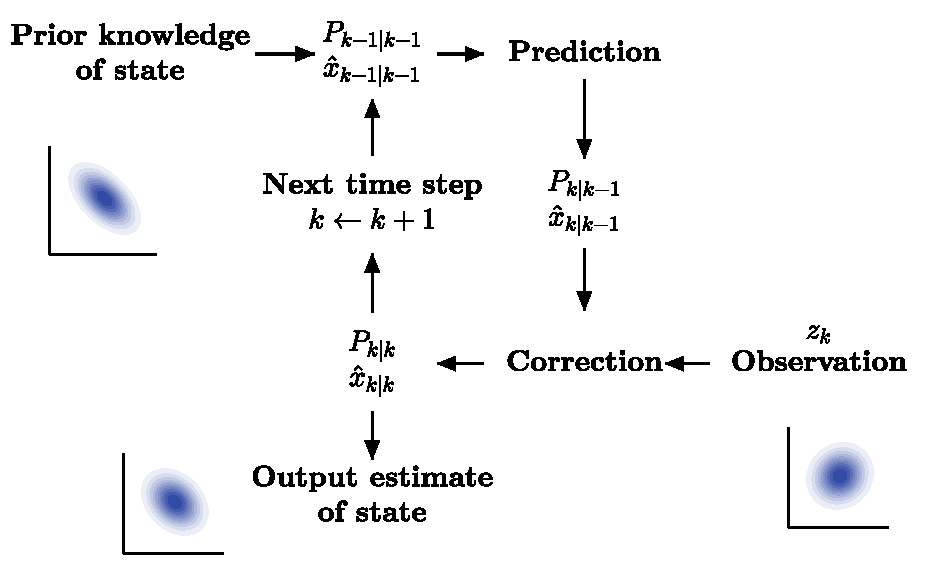
\includegraphics[width=0.9\textwidth]{../../Images/Étapes du filtre de Kalman avec équations.pdf}
	\caption{Schematic representation of the Kalman filter prediction/correction cycle. Each ellipsoid represents a confidence region associated with its corresponding Gaussian density.}\label{fig:Kalman_filter}
\end{figure}

\begin{algorithm}[!htb]
	\begin{algorithmic}
	\State{$\hat{x}_{k|k-1}=F_k\:\hat{x}_{k-1|k-1}+b_k^{(e)}$}\Comment{State prediction}
	\State{$P_{k|k-1}=F_k\:P_{k-1|k-1}\:F_k^\top+Q_k$}\Comment{Covariance prediction}
	\State{$y_k=z_k-\left(H_k\:\hat{x}_{k|k-1}+b_k^{(o)}\right)$}\Comment{Innovation}
	\State{$S_k=H_k\:P_{k|k-1}\:H_k^\top+R_k$}\Comment{Innovation covariance}
	\State{$K_k=P_{k|k-1}\:H_k^\top\:S_k^{-1}$}\Comment{Kalman gain}
	\State{$\hat{x}_{k|k}=\hat{x}_{k|k-1}+K_k\:y_k$}\Comment{State correction}
	\State{$P_{k|k}=(I-K_k\:H_k)\:P_{k|k-1}$}\Comment{Covariance correction}
	\end{algorithmic}\caption{Kalman Filter}\label{alg:Kalman_filter}
\end{algorithm}

\begin{remark}[Kalman state estimation]
	Under the Kalman assumptions, the PDF is Gaussian, and so every Bayesian estimator presented in \cref{sec:state_estimation} coincides with $\hat{x}_{k|k}$:
	\begin{equation}
		\hat{\psi}_{\mathrm{MMSE}}(\mathbf{z}_{1:k})=\hat{\psi}_{\mathrm{MMAE}}(\mathbf{z}_{1:k})=\hat{\psi}_{\mathrm{MAP}}(\mathbf{z}_{1:k})=\hat{x}_{k|k}
	\end{equation}

	However, since the above equations use a predictive prior, the ML estimator does not generally correspond to the corrected state.
\end{remark}

\begin{remark}[Precomputation of gains]
	Under the assumptions of \eqref{eq:Kalman_assumptions}, the matrices $P_{k|k-1}$, $K_k$ and $P_{k|k}$ depend only on the system matrices $F_k$, $H_k$, $Q_k$, $R_k$ and the initial covariance $P_0$, but not on the observations $z_k$. They can therefore be computed before any measurement is received.
\end{remark}

\subsubsection{Joseph's Formula}

In finite-precision arithmetic, the standard update $P_{k|k}=(I-K_k\:H_k)\:P_{k|k-1}$ may lose symmetry or positive definiteness due to rounding errors. Joseph's formula \cite{bib:Joseph,bib:Kalman-numerics} gives an alternative way to compute $P_{k|k}$ while ensuring that this property remains numerically satisfied:
\begin{equation}
	\begin{aligned}
	P_{k|k}&=(I-K_k\:H_k)\:P_{k|k-1}\\
	&=(I-K_k\:H_k)\:P_{k|k-1}-K_k\:S_k\:K_k^\top+K_k\:S_k\:K_k^\top\\
	&=(I-K_k\:H_k)\:P_{k|k-1}-(P_{k|k-1}\:H_k^\top\:S_k^{-1})\:S_k\:K_k^\top+K_k\:(H_k\:P_{k|k-1}\:H_k^\top+R_k)\:K_k^\top\\
	&=(I-K_k\:H_k)\:P_{k|k-1}-P_{k|k-1}\:H_k^\top\:K_k^\top+K_k\:H_k\:P_{k|k-1}\:H_k^\top\:K_k^\top+K_k\:R_k\:K_k^\top\\
	&=(I-K_k\:H_k)\:P_{k|k-1}-(I-K_k\:H_k)\:P_{k|k-1}\:H_k^\top\:K_k^\top+K_k\:R_k\:K_k^\top\\
	&=(I-K_k\:H_k)\:P_{k|k-1}(I-K_k\:H_k)^\top+K_k\:R_k\:K_k^\top\\
	\end{aligned}
\end{equation}

Under this more robust form, $P_{k|k}$ is SPSD as the sum of two SPSD matrices.

\subsection{Extended Kalman Filter}

The hypothesis that the evolution and observation functions are affine in $x_k$ is often too restrictive in practice. The extended Kalman filter (EKF) \cite{bib:EKF} relaxes this assumption by locally linearising $f_k$ and $h_k$ around the current state estimate via a first-order Taylor expansion.

Let $m,n\in\mathbb{N}^*$, let $f:\mathbb{R}^n\to\mathbb{R}^m$ be differentiable at some $a\in\mathbb{R}^n$. $f$ admits the following first-order expansion:
\begin{equation}
	\forall x\in\mathbb{R}^n,\:f(x)=f(a)+J_f(a)\:(x-a)+o(\|x-a\|_2)\label{eq:first_order_expansion}
\end{equation}
where $J_f(a)\in\mathcal{M}_{m,n}(\mathbb{R})$ is the Jacobian matrix of $f$ evaluated at $a$, and defined as:
\begin{equation}
	J_f\triangleq\frac{\partial f}{\partial x}=\begin{bmatrix}
	\dfrac{\partial f^{(1)}}{\partial x^{(1)}}&\cdots&\cdots&\dfrac{\partial f^{(1)}}{\partial x^{(n)}}\\
	\vdots&\ddots&\ddots&\vdots\\
	\dfrac{\partial f^{(m)}}{\partial x^{(1)}}&\cdots&\cdots&\dfrac{\partial f^{(m)}}{\partial x^{(n)}}
	\end{bmatrix}
\end{equation}
and $f^{(i)}$ and $x^{(j)}$ respectively denote the $i$-th and $j$-th component of $f$ and $x$.

Assuming that $f_k$ and $h_k$ are differentiable along the state trajectory, we can apply the first-order expansion \eqref{eq:first_order_expansion} to the evolution and observation model. Successive linearisations at each time step can then be used to apply the Kalman filter equations locally. The resulting algorithm is given by \Cref{alg:EKF}.

\begin{algorithm}[!htb]
	\begin{algorithmic}
	\State{$\tilde{F}_k=J_{f_k}\left(\hat{x}_{k-1|k-1}\right)$}\Comment{Evolution Jacobian}
	\State{$\hat{x}_{k|k-1}=f_k\left(\hat{x}_{k-1|k-1}\right)+b_k^{(e)}$}\Comment{State prediction}
	\State{$P_{k|k-1}=\tilde{F}_k\:P_{k-1|k-1}\:\tilde{F}_k^\top+Q_k$}\Comment{Covariance prediction}
	\State{$\tilde{H}_k=J_{h_k}\left(\hat{x}_{k|k-1}\right)$}\Comment{Observation Jacobian}
	\State{$y_k=z_k-\left(h_k\left(\hat{x}_{k|k-1}\right)+b_k^{(o)}\right)$}\Comment{Innovation}
	\State{$S_k=\tilde{H}_k\:P_{k|k-1}\:\tilde{H}_k^\top+R_k$}\Comment{Innovation covariance}
	\State{$K_k=P_{k|k-1}\:\tilde{H}_k^\top\:S_k^{-1}$}\Comment{Kalman gain}
	\State{$\hat{x}_{k|k}=\hat{x}_{k|k-1}+K_k\:y_k$}\Comment{State correction}
	\State{$P_{k|k}=(I-K_k\:\tilde{H}_k)\:P_{k|k-1}$}\Comment{Covariance correction}
	\end{algorithmic}\caption{Extended Kalman Filter}\label{alg:EKF}
\end{algorithm}

While less restrictive than the standard Kalman filter, the EKF is suboptimal for three reasons:
\begin{itemize}
	\item First, $f_k$ and $h_k$ must be differentiable along the state trajectory, which excludes discontinuous or piecewise-defined models.
	\item Second, the linearisation in \eqref{eq:first_order_expansion} neglects higher-order terms of the Taylor expansion, which introduces an approximation error that grows with the degree of nonlinearity of $f_k$ and $h_k$. This error increases over time as it propagates through the equations of the Kalman filter due to the sequential formulation.
	\item Finally, it relies on Gaussian assumptions and thus fails to handle multimodal or heavy-tailed distributions, as does its affine counterpart.
\end{itemize}

\subsection{Other Suboptimal Kalman Filters}

\subsubsection{Iterative and Higher-Order EKF}

The iterative EKF (IEKF) \cite{bib:IEKF} improves upon the EKF correction step by iteratively re-linearising $h_k$ around successive state estimates within the same measurement update, while keeping the prediction step unchanged. Starting from the initialisation $\hat{x}_{k|k}^{(0)}=\hat{x}_{k|k-1}$, each iteration produces a new $\hat{x}_{k|k}^{(i)}$ by repeating the correction step from the predicted state, with the Jacobian evaluated at the latest estimate. This is done until:
\begin{equation}
	\left\|\hat{x}_{k|k}^{(i)}-\hat{x}_{k|k}^{(i-1)}\right\|_2\leq\varepsilon
\end{equation}
for some $\varepsilon>0$, or a maximum number of iterations is reached. The corrected state and covariance matrix are then defined as the result of the last loop.

This procedure is equivalent to performing a Gauss-Newton descent \cite{bib:IEKF-Gauss-Newton} on the posterior density maximisation problem, and converges to the MAP estimator under Gaussian assumptions. It reduces the linearisation error of the correction step when $h_k$ is strongly non-linear, at the cost of several Jacobian evaluations per time step.

The second-order EKF (SO-EKF) \cite{bib:SO-EKF} can also be used to extend the linearisation \eqref{eq:first_order_expansion} to second-order terms via the Hessians of $f_k$ and $h_k$, which reduces the approximation error for highly nonlinear models. However, it requires computing and storing the Hessian matrices of $f_k$ and $h_k$ at each time step, making it computationally prohibitive in high dimensions.

\subsubsection{Unscented Kalman Filter}

Rather than linearising the model, the unscented Kalman filter (UKF) \cite{bib:UKF} propagates a small deterministic set of points through the non-linear functions themselves. Let $d\in\mathbb{N}^*$, and let $X$ be a random vector of $\mathbb{R}^d$ with mean $\mu$ and covariance $P\succ0$. The $2d+1$ sigma points associated with $X$, and their weights, are:
\begin{equation}
	\left\{\begin{aligned}
	\mathcal{X}^{(0)}&\triangleq\mu,&\quad W^{(0)}&\triangleq\frac{\lambda}{d+\lambda}\\
	\mathcal{X}^{(\pm i)}&\triangleq\mu\pm\sqrt{d+\lambda}\:(A)_i,&\quad W^{(\pm i)}&\triangleq\frac{1}{2(d+\lambda)},\:i\in[\![1,d]\!]
	\end{aligned}\right.
\end{equation}
where $A$ is a Cholesky factor \cite{bib:matrix-computations} of $P$, $(A)_i$ is its $i$-th column, and $\lambda>-d$ is a scaling parameter. In particular, the weights are independent of $X$ and add up to $1$.

For a function $\varphi$, the first and second moments of $\varphi(X)$ can then be approximated by the weighted moments of the images of the sigma points:
\begin{equation}
	\left\{\begin{aligned}
	\hat{\varphi}&\triangleq\sum_{i=-d}^{d}W^{(i)}\:\varphi\left(\mathcal{X}^{(i)}\right)\\
	\hat{P}&\triangleq\sum_{i=-d}^{d}W^{(i)}\left(\varphi\left(\mathcal{X}^{(i)}\right)-\hat{\varphi}\right)\left(\varphi\left(\mathcal{X}^{(i)}\right)-\hat{\varphi}\right)^\top
	\end{aligned}\right.
\end{equation}

This procedure is known as the unscented transform \cite{bib:unscented}, and is applied twice per time step by the UKF. It is first used with $\mu=\hat{x}_{k-1|k-1}$, $P=P_{k-1|k-1}$ and $\varphi=f_k$ to compute the predicted state, then with $\mu=\hat{x}_{k|k-1}$, $P=P_{k|k-1}$ and $\varphi=h_k$ to obtain the predicted observation and thus the innovation. In both cases, $Q_k$ and $R_k$ are added to the transformed covariance $\hat{P}$, as in \Cref{alg:EKF}, to account for evolution and observation uncertainty.

This removes the linearisation shortcomings of the EKF, at the cost of $2d_x+1$ evaluations of $f_k$ and $h_k$ per time step. A square-root formulation \cite{bib:SRUKF} propagates a factor of the covariance rather than the covariance itself, which preserves its symmetry and positive definiteness throughout the recursion. However, the UKF still relies on the Gaussian assumption, the posterior remaining summarised by a mean and a covariance matrix.

\subsubsection{Ensemble Kalman Filter}

The ensemble Kalman filter (EnKF) \cite{bib:EnKF} avoids both the local linearisation of the EKF and the deterministic sigma-point approximation of the UKF. Instead, the state distribution is represented by a set of $N\in\mathbb{N}^*$ samples $\left(x_{k|k}^{(1)},\dots,x_{k|k}^{(N)}\right)$, which are propagated through the true evolution and observation functions.

For two sets $\mathbf{X}\triangleq(X^{(1)},\dots,X^{(N)})$ and $\mathbf{Z}\triangleq(Z^{(1)},\dots,Z^{(N)})$, we let:
\begin{equation}
	\left\{\begin{aligned}
	\hat{X}&\triangleq\frac{1}{N}\sum_{i=1}^NX^{(i)},\qquad
	\hat{Z}\triangleq\frac{1}{N}\sum_{i=1}^NZ^{(i)}\\
	\hat{P}_{\mathbf{XZ}}&\triangleq\frac{1}{N-1}\sum_{i=1}^N\left(X^{(i)}-\hat{X}\right)\left(Z^{(i)}-\hat{Z}\right)^\top
	\end{aligned}\right.
\end{equation}

Each predicted sample $x_{k|k-1}^{(i)}$ is obtained by propagating the corresponding sample $x_{k-1|k-1}^{(i)}$ through $f_k$. The predicted observation $z_k^{(i)}$ is then computed using $h_k$.

The approximate Kalman gain is defined as:
\begin{equation}
	\hat{K}_k\triangleq\hat{P}_{\mathbf{X}_{k|k-1}\mathbf{Z}_k}\:\left(\hat{P}_{\mathbf{Z}_k\mathbf{Z}_k}+R_k\right)^{-1}
\end{equation}
where $\mathbf{X}_{k|k-1}$ is the predicted sample set, and $\mathbf{Z}_k$ is the predicted observation set. Finally, each corrected sample $x_{k|k}^{(i)}$ is computed from its associated predicted sample through a standard Kalman update, using $\hat{K}_k$ in place of the exact gain.

The computational cost of the EnKF is primarily determined by the value of $N$ instead of the dimensions $d_x$ and $d_z$. It is therefore particularly attractive for high-dimensional systems, such as those encountered in meteorological and oceanographic data assimilation \cite{bib:EnKF-atmosphere}.

It should be noted that, while the EnKf is more flexible than its counterparts, the correction step remains a Kalman update based on the empirical mean and covariance matrix of the sample set. As a result, it may provide a poor approximation when the PDF is strongly non-Gaussian.
